\documentclass[a4paper, 12pt, titlepage]{article}
\usepackage[utf8]{inputenc}
\usepackage[english]{babel}
\usepackage[]{parskip}
\usepackage{graphicx}
\usepackage{xcolor}
\usepackage{paralist} % compactitem
\usepackage{csquotes}
\usepackage{wrapfig}
\usepackage{subfig}
\usepackage{csvsimple} % csv tables

% Title spacing
\usepackage{titlesec}
\titlespacing*{\section}{0pt}{0pt}{0pt}
\titlespacing*{\subsection}{0pt}{-5pt}{-5pt}
\titlespacing*{\subsubsection}{0pt}{0pt}{0pt}

% Citations
\usepackage[
  style=ieee,
  citecounter,
  labelnumber,
  backend=biber,
  bibencoding=utf8,
  sorting=none
]{biblatex}
\addbibresource{references.bib}

% Code blocks
\usepackage{listings}
\definecolor{codegreen}{rgb}{0,0.6,0}
\definecolor{codegray}{rgb}{0.5,0.5,0.5}
\definecolor{codepurple}{rgb}{0.58,0,0.82}
\definecolor{backcolour}{rgb}{0.95,0.95,0.92}
\lstdefinestyle{mystyle}{
  backgroundcolor=\color{backcolour},
  commentstyle=\color{codegreen},
  keywordstyle=\color{magenta},
  numberstyle=\tiny\color{codegray},
  stringstyle=\color{codepurple},
  basicstyle=\ttfamily\tiny,
  breakatwhitespace=false,
  breaklines=true,
  captionpos=b,
  keepspaces=false,
  numbersep=5pt,
  showspaces=false,
  showstringspaces=false,
  showtabs=false,
  tabsize=2
}
\lstset{style=mystyle}

% Custom commands
% Referencing
\newcommand{\figRef}[1]{Figure \ref{#1}}
\newcommand{\tabRef}[1]{Table \ref{#1}}
\newcommand{\eqRef}[1]{(\ref{#1})}
% Reading data from files
%\newcommand{\knnData}[1]{\DTLfetch{knndata}{key}{#1}{value}}
%\newcommand{\neighborhoodData}[1]{\DTLfetch{neighborhooddata}{key}{#1}{value}}
%\newcommand{\perceptronData}[1]{\DTLfetch{perceptrondata}{key}{#1}{value}}
% Values
\newcommand{\digitwidth}{0.08\textwidth}
\newcommand{\doubledigitwidth}{0.15\textwidth}

\title{EECE6036 - Homework 3}
\author{Wayne Stegner}
\date{\today}

\begin{document}
  \maketitle
  \section{Problem 1}
  \subsection{Problem Summary}
  \par The goal of this problem is to create a multi-layer feed-forward neural
  network for classification of the MNIST dataset.
  The network was trained using gradient descent with back-propagation with
  momentum, and is trainable for arbitrary amounts and sizes of hidden layers.
  During training, the loss is calculated using $J_{2}$ loss with threshold
  values.
  For performance measurement, the loss is calculated as $1 - hit\_rate$ using
  winner-take-all on the output layer to define the predicted class.

  \subsection{Results}
  \subsubsection{System Description}
  \par \tabRef{tab:class_param} shows the hyper-parameters used in training the
  classifier.
  These hyper-parameters were found empirically, considering both minimizing
  the final loss and training time.
  More work can to find more optimal hyper-parameters, but this set of
  hyper-parameters produces pretty good results.
  \begin{table}[htb]
    \centering
    \vspace{-12pt}
    \caption{Classifier Training Hyper-Parameters}
    \vspace{-12pt}
    \csvautotabular{data/class_parameters.csv}
    \label{tab:class_param}
    \vspace{-12pt}
  \end{table}
  \par Weight initialization is done randomly on a uniform distribution between
  $(-a, +a)$ where $a = \sqrt(\frac{6}{N_{source} + N_{target}})$, and
  $N_{source}$ and $N_{target}$ are the numbers of neurons on the source and
  target layers respectively.
  \par The network utilizes early stopping by monitoring a validation set,
  which consists of 1000 training points that are set aside before training.
  If the validation loss does not improve for $patience$ steps (1 step = 10
  epochs), training halts.
  The validation is considered improved if the validation is $es\_delta$ lower
  than the previous improved validation loss.
  The weights used by the final network are the weights from the epoch with the
  lowest validation loss.
  To improve the frequency of checking for early stopping, the network only
  uses 1000 training points per epoch.

  \subsubsection{Network Results}
  \par Throughout the duration of training, the loss of the training and
  validation sets was tracked every 10 epochs.
  \figRef{fig:class_loss} shows a plot of the loss values while training the
  classifier.
  The vertical line designates the point where the validation error is
  minimized, which occurs at epoch
  \input{data/class_best_epoch.dat}\unskip{}.
  The weights at that epoch are the weights used in the final network, where
  the test loss is \input{data/class_test_loss.dat}\unskip{}.
  \begin{figure}[htb]
    \centering
    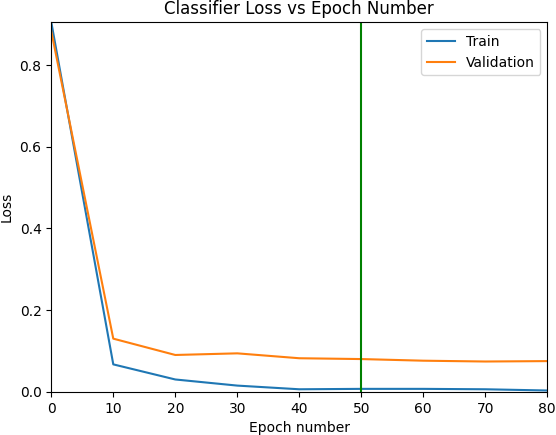
\includegraphics[width=0.5\textwidth]{images/class_loss.png}
    \caption{Training and validation loss of the classifier.}
    \label{fig:class_loss}
  \end{figure}
  \par \figRef{fig:conf} shows the confusion matrices for the train and
  test sets using the weights from the best epoch.
  \begin{figure}[htb]
    \centering
    \subfloat[][]{
      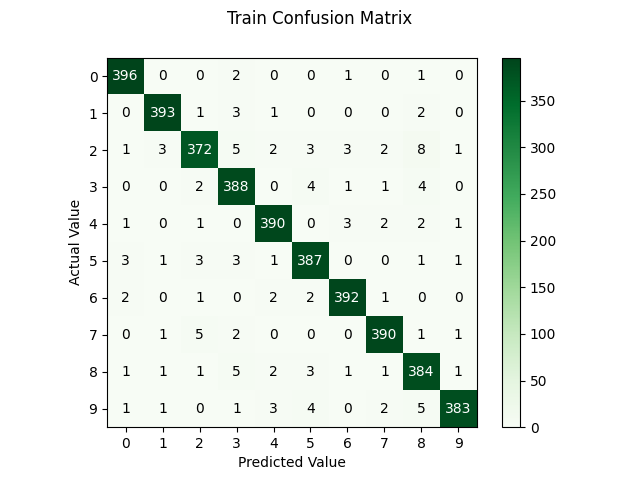
\includegraphics[width=0.48\textwidth]{images/train_conf_mat.png}
      \label{fig:conf_train}
    }
    \subfloat[][]{
      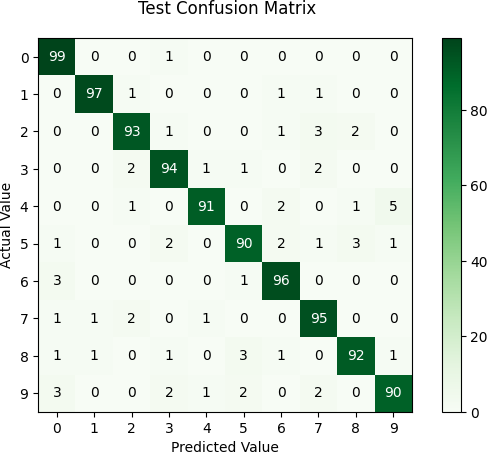
\includegraphics[width=0.48\textwidth]{images/test_conf_mat.png}
      \label{fig:conf_test}
    }
    \caption{Confusion matrices of the train and test sets.}
    \label{fig:conf}
  \end{figure}

  \subsection{Discussion and Analysis of Results}
  \par Overall, the results look pretty good.
  The best weights happen pretty early at epoch
  \input{data/class_best_epoch.dat}\unskip{} and get a fairly low loss of
  \input{data/class_test_loss.dat}\unskip{}.
  While testing hyper-parameters, it was observed that when $es\_delta$ is set
  to 0 and $patience$ is increased to around 5, the test loss would sometimes
  get as low as 0.05, but that generally occurred after several hundred epochs
  and is also dependent on weight initialization numbers and dataset shuffling
  during training.
  With the early stopping hyper-parameters used by this model, it sacrifices
  some performance, but it trains significantly faster, making these
  hyper-parameters ideal for implementing and troubleshooting the network from
  scratch.
  \par The diagonal of the confusion matrices in \figRef{fig:conf} is very
  dark, with hardly any coloring in the incorrect boxes.
  Many of the incorrect classifications are in two classes which look similar.
  For example, \figRef{fig:conf_train} shows four 9s classified as 4s and five
  4s classified as 9s.
  This mix-up makes a lot of sense, because the shapes of 4s and 9s tend to be
  similar, especially with some of the sloppy handwriting in MNIST.

  \subsection{Conclusion}
  \par This multi-layer feed-forward neural network classifier is able to
  effectively classify the MNIST dataset given in this problem.
  While the results are certainly not state-of-the-art, the trained network
  classifies over 90\% of the test set digits correctly.
  Further testing in optimizing the hyper-parameters of the network can help to
  improve the accuracy even further.

  \pagebreak
  \section{Problem 2}
  \subsection{Problem Summary}
  \par The goal of this problem is to create a multi-layer feed-forward neural
  network similar to Problem 1, except in this case it will be trained to be an
  autoencoder.
  This network has the same features as the network in Problem 1, except the
  performance measurement is calculated using $J_{2}$ loss instead of
  $1 - hit\_rate$.
  Additionally, winner-take-all is not used in the output layer, because it
  does not make sense in the context of an autoencoder.

  \subsection{Results}
  \subsubsection{System Description}
  \par \tabRef{tab:auto_param} shows the hyper-parameters used in training
  the autoencoder.
  As with the classifier, these hyper-parameters were found empirically with
  the same consideration for minimizing final loss and training time.
  \begin{table}[htb]
    \centering
    \caption{Autoencoder Training Hyper-Parameters}
    \vspace{-12pt}
    \csvautotabular{data/auto_parameters.csv}
    \label{tab:auto_param}
    \vspace{-12pt}
  \end{table}
  \par The weight initialization process is the same as in Problem 1, as are
  the processes for allocating the validation set and applying early stopping.

  \subsubsection{Network Results}
  \par Throughout the duration of training, the loss of the training and
  validation sets was tracked every 10 epochs.
  \figRef{fig:auto_loss} shows a plot of the loss values while training the
  autoencoder.
  The vertical line designates the point where the validation error is
  minimized, which occurs at epoch
  \input{data/auto_best_epoch.dat}\unskip{}.
  The weights at that epoch are the weights used in the final network, where
  the test loss is \input{data/auto_test_loss.dat}\unskip{}.
  \begin{figure}[htb]
    \centering
    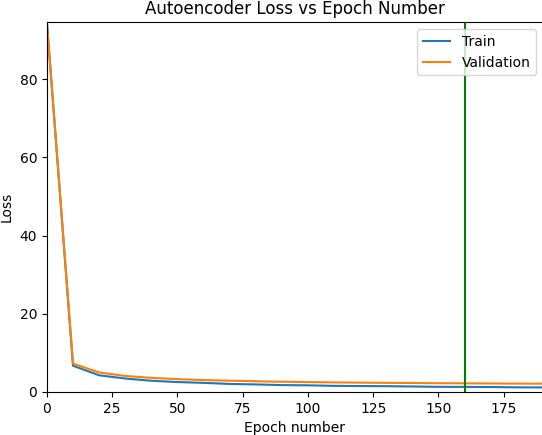
\includegraphics[width=0.5\textwidth]{images/auto_loss.png}
    \caption{Training and validation loss of the autoencoder.}
    \label{fig:auto_loss}
  \end{figure}
  \par After training, the loss in each class was measured.
  \figRef{fig:bar} shows the loss of each class for the train and
  test sets using the weights from the best epoch.
  \begin{figure}[htb]
    \centering
    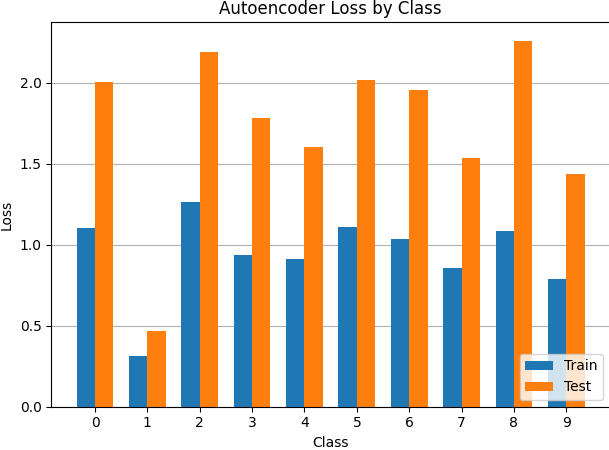
\includegraphics[width=0.5\textwidth]{images/loss_bar_plot.png}
    \caption{Loss of each class of the train and test sets.}
    \label{fig:bar}
  \end{figure}

  \subsubsection{Features}
  \par After training, the features learned by 20 arbitrary neurons in the
  hidden layer of both the classifier and autoencoder were observed by
  normalizing the weights from 0 to 1 and then displaying them like an image.
  The images are mapped so 1 is white and 0 is black.
  \figRef{fig:class_feat} shows the features of the classifier, and
  \figRef{fig:auto_feat} shows the features of the autoencoder.
  \begin{figure}[htb]
    \begin{minipage}{0.45\textwidth}
      \centering
            \subfloat[][]{
        
\includegraphics[width=\doubledigitwidth]
        {images/class_feat/feat_00.png}
      }
      \subfloat[][]{
        
\includegraphics[width=\doubledigitwidth]
        {images/class_feat/feat_01.png}
      }
      \subfloat[][]{
        
\includegraphics[width=\doubledigitwidth]
        {images/class_feat/feat_02.png}
      }
      \subfloat[][]{
        
\includegraphics[width=\doubledigitwidth]
        {images/class_feat/feat_03.png}
      }
      \subfloat[][]{
        
\includegraphics[width=\doubledigitwidth]
        {images/class_feat/feat_04.png}
      } \\
      \subfloat[][]{
        
\includegraphics[width=\doubledigitwidth]
        {images/class_feat/feat_05.png}
      }
      \subfloat[][]{
        
\includegraphics[width=\doubledigitwidth]
        {images/class_feat/feat_06.png}
      }
      \subfloat[][]{
        
\includegraphics[width=\doubledigitwidth]
        {images/class_feat/feat_07.png}
      }
      \subfloat[][]{
        
\includegraphics[width=\doubledigitwidth]
        {images/class_feat/feat_08.png}
      }
      \subfloat[][]{
        
\includegraphics[width=\doubledigitwidth]
        {images/class_feat/feat_09.png}
      } \\
      \subfloat[][]{
        
\includegraphics[width=\doubledigitwidth]
        {images/class_feat/feat_10.png}
      }
      \subfloat[][]{
        
\includegraphics[width=\doubledigitwidth]
        {images/class_feat/feat_11.png}
      }
      \subfloat[][]{
        
\includegraphics[width=\doubledigitwidth]
        {images/class_feat/feat_12.png}
      }
      \subfloat[][]{
        
\includegraphics[width=\doubledigitwidth]
        {images/class_feat/feat_13.png}
      }
      \subfloat[][]{
        
\includegraphics[width=\doubledigitwidth]
        {images/class_feat/feat_14.png}
      } \\
      \subfloat[][]{
        
\includegraphics[width=\doubledigitwidth]
        {images/class_feat/feat_15.png}
      }
      \subfloat[][]{
        
\includegraphics[width=\doubledigitwidth]
        {images/class_feat/feat_16.png}
      }
      \subfloat[][]{
        
\includegraphics[width=\doubledigitwidth]
        {images/class_feat/feat_17.png}
      }
      \subfloat[][]{
        
\includegraphics[width=\doubledigitwidth]
        {images/class_feat/feat_18.png}
      }
      \subfloat[][]{
        
\includegraphics[width=\doubledigitwidth]
        {images/class_feat/feat_19.png}
      }

      \caption{Classifier features.}
      \label{fig:class_feat}
    \end{minipage}
    \hfill
    \begin{minipage}{0.45\textwidth}
      \centering
            \subfloat[][]{
        
\includegraphics[width=\doubledigitwidth]
        {images/auto_feat/feat_00.png}
      }
      \subfloat[][]{
        
\includegraphics[width=\doubledigitwidth]
        {images/auto_feat/feat_01.png}
      }
      \subfloat[][]{
        
\includegraphics[width=\doubledigitwidth]
        {images/auto_feat/feat_02.png}
      }
      \subfloat[][]{
        
\includegraphics[width=\doubledigitwidth]
        {images/auto_feat/feat_03.png}
      }
      \subfloat[][]{
        
\includegraphics[width=\doubledigitwidth]
        {images/auto_feat/feat_04.png}
      } \\
      \subfloat[][]{
        
\includegraphics[width=\doubledigitwidth]
        {images/auto_feat/feat_05.png}
      }
      \subfloat[][]{
        
\includegraphics[width=\doubledigitwidth]
        {images/auto_feat/feat_06.png}
      }
      \subfloat[][]{
        
\includegraphics[width=\doubledigitwidth]
        {images/auto_feat/feat_07.png}
      }
      \subfloat[][]{
        
\includegraphics[width=\doubledigitwidth]
        {images/auto_feat/feat_08.png}
      }
      \subfloat[][]{
        
\includegraphics[width=\doubledigitwidth]
        {images/auto_feat/feat_09.png}
      } \\
      \subfloat[][]{
        
\includegraphics[width=\doubledigitwidth]
        {images/auto_feat/feat_10.png}
      }
      \subfloat[][]{
        
\includegraphics[width=\doubledigitwidth]
        {images/auto_feat/feat_11.png}
      }
      \subfloat[][]{
        
\includegraphics[width=\doubledigitwidth]
        {images/auto_feat/feat_12.png}
      }
      \subfloat[][]{
        
\includegraphics[width=\doubledigitwidth]
        {images/auto_feat/feat_13.png}
      }
      \subfloat[][]{
        
\includegraphics[width=\doubledigitwidth]
        {images/auto_feat/feat_14.png}
      } \\
      \subfloat[][]{
        
\includegraphics[width=\doubledigitwidth]
        {images/auto_feat/feat_15.png}
      }
      \subfloat[][]{
        
\includegraphics[width=\doubledigitwidth]
        {images/auto_feat/feat_16.png}
      }
      \subfloat[][]{
        
\includegraphics[width=\doubledigitwidth]
        {images/auto_feat/feat_17.png}
      }
      \subfloat[][]{
        
\includegraphics[width=\doubledigitwidth]
        {images/auto_feat/feat_18.png}
      }
      \subfloat[][]{
        
\includegraphics[width=\doubledigitwidth]
        {images/auto_feat/feat_19.png}
      }

      \caption{Autoencoder features.}
      \label{fig:auto_feat}
    \end{minipage}
  \end{figure}

  \subsubsection{Sample Outputs}
  \par After training, the outputs of eight random data points from the test
  set were fed reconstructed the autoencoder, meaning the input data point was
  presented to the network and the output "prediction" was obtained.
  \figRef{fig:samples} shows the original and reconstructed images.
  \begin{figure}[htb]
    \centering
        \subfloat[][]{
      \rotatebox{90}{\tiny Original}
      
\includegraphics[width=\digitwidth]
        {images/auto_samples/orig_0.png}
    }
    \subfloat[][]{
      
\includegraphics[width=\digitwidth]
        {images/auto_samples/orig_1.png}
    }
    \subfloat[][]{
      
\includegraphics[width=\digitwidth]
        {images/auto_samples/orig_2.png}
    }
    \subfloat[][]{
      
\includegraphics[width=\digitwidth]
        {images/auto_samples/orig_3.png}
    }
    \subfloat[][]{
      
\includegraphics[width=\digitwidth]
        {images/auto_samples/orig_4.png}
    }
    \subfloat[][]{
      \includegraphics[width=\digitwidth]
        {images/auto_samples/orig_5.png}
    }
    \subfloat[][]{
      \includegraphics[width=\digitwidth]
        {images/auto_samples/orig_6.png}
    }
    \subfloat[][]{
      \includegraphics[width=\digitwidth]
        {images/auto_samples/orig_7.png}
    }\\
    \subfloat[][]{
      \rotatebox{90}{\tiny Reconstructed}
      \includegraphics[width=\digitwidth]
        {images/auto_samples/pred_0.png}
    }
    \subfloat[][]{
      \includegraphics[width=\digitwidth]
        {images/auto_samples/pred_1.png}
    }
    \subfloat[][]{
      \includegraphics[width=\digitwidth]
        {images/auto_samples/pred_2.png}
    }
    \subfloat[][]{
      \includegraphics[width=\digitwidth]
        {images/auto_samples/pred_3.png}
    }
    \subfloat[][]{
      \includegraphics[width=\digitwidth]
        {images/auto_samples/pred_4.png}
    }
    \subfloat[][]{
      \includegraphics[width=\digitwidth]
        {images/auto_samples/pred_5.png}
    }
    \subfloat[][]{
      \includegraphics[width=\digitwidth]
        {images/auto_samples/pred_6.png}
    }
    \subfloat[][]{
      \includegraphics[width=\digitwidth]
        {images/auto_samples/pred_7.png}
    }

    \caption{Original (top) and reconstructed (bottom) data points.}
    \label{fig:samples}
  \end{figure}

  \subsection{Discussion and Analysis of Results}
  \par Overall, the results look pretty good.
  The autoencoder takes longer to train, with its best weights occurring at
  epoch \input{data/auto_best_epoch.dat}\unskip{} with a loss of
  \input{data/auto_test_loss.dat}\unskip{}.
  In \figRef{fig:bar}, the loss for the 1s is particularly salient because it
  is drastically lower than the other classes loss values.
  This makes sense because a 1 is simply a straight line, so it should be quite
  simple to recognize and then reconstruct.
  While none of the loss values are as noticeably high as 1's loss is low,
  classes 2, 8, and 5 all have loss values above 2.5.
  I do not have any intuition as to why those numbers have the highest loss,
  but those digits are kind of similar in the sense that a 2 is roughly a
  backward 5, and stacking a 2 on top of a 5 roughly makes an 8.
  At first, I was surprised that 6 has a higher loss than 9, because 6 is just
  an upside-down 9, but it makes sense that 5 and 6 have similar features and
  ended up having similar loss values.
  \par The features in \figRef{fig:class_feat} and \figRef{fig:auto_feat} are
  somewhat difficult to interpret.
  Between the two feature sets, there is a trend where the center of the image
  appears to have some distinct patterns, while the edge of the image is either
  somewhat uniform gray or random TV static.
  This trend makes sense because the digits in the images tended to be
  mostly centered, so the edge pixels mostly contained 0.
  When the presented input is 0, the weight delta is 0 according to the
  back-propagation formula, meaning that the edge of the images did not get
  updated as much as the center of the image.
  In \figRef{fig:class_feat}, the shapes generally seem to be lines or curves,
  while in \figRef{fig:auto_feat} the features look like a bunch of dark dots
  with a few brighter spots.


  \subsection{Conclusion}
  \par This multi-layer feed-forward neural network autoencoder is able to
  effectively reconstruct digits from the MNIST dataset.
  Further testing in optimizing the hyper-parameters of the network can help to
  improve the reconstruction accuracy even further.

  \pagebreak
  \appendix
  \section{Code}
  \subsection{\texttt{settings.py}}
  \lstinputlisting[language=python]{"code/settings.py"}
  \subsection{\texttt{dataset.py}}
  \lstinputlisting[language=python]{"code/dataset.py"}
  \subsection{\texttt{layer.py}}
  \lstinputlisting[language=python]{"code/layer.py"}
  \subsection{\texttt{output\_layer.py}}
  \lstinputlisting[language=python]{"code/output_layer.py"}
  \subsection{\texttt{hidden\_layer.py}}
  \lstinputlisting[language=python]{"code/hidden_layer.py"}
  \subsection{\texttt{mlp.py}}
  \lstinputlisting[language=python]{"code/mlp.py"}
  \subsection{\texttt{classifier.py}}
  \lstinputlisting[language=python]{"code/classifier.py"}
  \subsection{\texttt{autoencoder.py}}
  \lstinputlisting[language=python]{"code/autoencoder.py"}
  \subsection{\texttt{test\_classifier.py}}
  \lstinputlisting[language=python]{"code/test_classifier.py"}
  \subsection{\texttt{test\_autoencoder.py}}
  \lstinputlisting[language=python]{"code/test_autoencoder.py"}
  \subsection{\texttt{features.py}}
  \lstinputlisting[language=python]{"code/features.py"}

\end{document}
